\documentclass[11pt]{article}
\usepackage[margin=1in]{geometry}
\usepackage{amsmath,amssymb,amsthm}
\usepackage{algorithm}
\usepackage{algpseudocode}
\usepackage{tikz}
\usetikzlibrary{arrows.meta,positioning,calc}

\newcommand{\R}{\mathbb{R}}
\newcommand{\N}{\mathcal{N}}
\newcommand{\xclean}{x}
\newcommand{\xpert}{x_\varepsilon}
\newcommand{\eps}{\varepsilon}
\newcommand{\layerl}{\ell}

\newtheorem{proposition}{Proposition}
\newtheorem{definition}{Definition}
\newtheorem{remark}{Remark}

\title{Joining Variables Across Three Network Copies\\in VHAGaR Transfer Mode}
\author{Research Notes}
\date{}

\begin{document}
\maketitle

%----------------------------------------------------------------------
\section{Setup and Notation}
%----------------------------------------------------------------------

In VHAGaR transfer mode we encode three network copies\footnote{%
Four when \texttt{n1\_p\_mode=true}; here we focus on the common case
$\{N_1(x),\; N_2(x),\; N_2(x_\varepsilon)\}$.}
sharing the same input $x\in[0,1]^d$ and perturbation
$x_\varepsilon = x + e$, $\|e\|_\infty\le\eps$:

\begin{center}
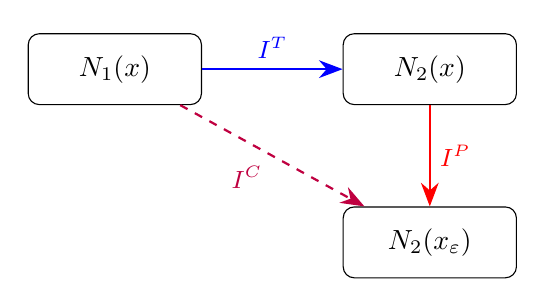
\begin{tikzpicture}[
    box/.style={draw, rounded corners, minimum width=2.2cm, minimum height=0.9cm, align=center},
    arr/.style={-{Stealth[length=3mm]}, thick},
]
  \node[box] (n1x)  at (0,0)   {$N_1(x)$};
  \node[box] (n2x)  at (4,0)   {$N_2(x)$};
  \node[box] (n2xp) at (4,-2.2) {$N_2(x_\varepsilon)$};

  \draw[arr, blue]  (n1x)  -- node[above]{\small $I^T$} (n2x);
  \draw[arr, red]   (n2x)  -- node[right]{\small $I^P$} (n2xp);
  \draw[arr, purple, dashed] (n1x) -- node[below left]{\small $I^C$} (n2xp);
\end{tikzpicture}
\end{center}

\noindent
where the interval types are:
\begin{itemize}
    \item \textbf{Transfer interval} $I^T$ (blue): bounds the difference
          $z^{N_2}_\layerl(x) - z^{N_1}_\layerl(x)$ due to different weights $W_2 \ne W_1$.
          Currently implemented in \texttt{transfer\_interval\_constraints}.
    \item \textbf{Perturbation interval} $I^P$ (red): bounds the difference
          $z^{N_2}_\layerl(x_\varepsilon) - z^{N_2}_\layerl(x)$ due to $\|e\|_\infty\le\eps$.
          Currently implemented in \texttt{perturbed\_interval\_constraints}.
    \item \textbf{Composed interval} $I^C$ (purple, dashed): bounds
          $z^{N_2}_\layerl(x_\varepsilon) - z^{N_1}_\layerl(x)$ directly.
          \emph{Not yet implemented}---this is the main proposal.
\end{itemize}

\paragraph{Per-layer notation.}
For neuron $i$ at layer $\layerl$ (post-activation), denote:
\begin{align}
    a^{N_1}_{\layerl,i} &\;=\; \sigma\bigl(z^{N_1}_{\layerl,i}(x)\bigr),
    &
    a^{N_2}_{\layerl,i} &\;=\; \sigma\bigl(z^{N_2}_{\layerl,i}(x)\bigr),
    &
    \tilde{a}^{N_2}_{\layerl,i} &\;=\; \sigma\bigl(z^{N_2}_{\layerl,i}(x_\varepsilon)\bigr),
\end{align}
where $\sigma(\cdot) = \max(0,\cdot)$ is the ReLU. In the MIP, these correspond to the
\texttt{x\_rect} variables with prefixes \texttt{n1\_org}, \texttt{n2\_org}, \texttt{n2\_pert}.

The existing interval constraints enforce, at every ReLU layer $\layerl$:
\begin{align}
    a^{N_2}_{\layerl,i} &\;\in\; \bigl[a^{N_1}_{\layerl,i} + I^T_{\layerl,i,\text{down}},\;\;
                                          a^{N_1}_{\layerl,i} + I^T_{\layerl,i,\text{up}}\bigr],
    \label{eq:transfer}\\[4pt]
    \tilde{a}^{N_2}_{\layerl,i} &\;\in\; \bigl[a^{N_2}_{\layerl,i} + I^P_{\layerl,i,\text{down}},\;\;
                                                  a^{N_2}_{\layerl,i} + I^P_{\layerl,i,\text{up}}\bigr].
    \label{eq:perturbed}
\end{align}


%======================================================================
\section{Composed Interval $I^C$: Full Treatment}
\label{sec:composed}
%======================================================================

\subsection{Motivation}
\label{sec:composed:motivation}

The existing interval machinery provides two \emph{pairwise} links:
\begin{itemize}
    \item $I^T$: \; $N_1(x) \longleftrightarrow N_2(x)$ \quad
          (different weights, same input);
    \item $I^P$: \; $N_2(x) \longleftrightarrow N_2(x_\varepsilon)$ \quad
          (same weights, different input).
\end{itemize}
Together they form a \emph{chain} $N_1(x) \to N_2(x) \to N_2(x_\varepsilon)$.
Every feasible point in the MIP must satisfy \emph{both} links, yet Gurobi
sees them as separate constraint families---it cannot exploit transitivity
across them unless we make it explicit.

The composed interval $I^C$ closes this triangle by providing a \emph{direct}
bound on the difference $\tilde{a}^{N_2}_\layerl - a^{N_1}_\layerl$
between the first and last network copies.
This adds redundant-but-useful constraints that:
\begin{enumerate}
    \item Give Gurobi a direct bound between the copies that are farthest apart
          in the encoding, cutting across the intermediate $N_2(x)$ variables.
    \item Enable variable elimination or LP relaxation when the composed
          interval is tight (Sections~\ref{sec:merging}--\ref{sec:hybrid}).
    \item Are \emph{free} to compute---interval propagation is $O(n^2)$ per layer,
          negligible compared to MIP solving time.
\end{enumerate}

\subsection{Formal Definition}
\label{sec:composed:def}

\begin{definition}[Composed difference]
For each layer $\layerl$ and neuron $i$, define the \emph{composed difference}
\begin{equation}
    \Delta^C_{\layerl,i}
    \;\stackrel{\text{def}}{=}\;
    \tilde{a}^{N_2}_{\layerl,i} - a^{N_1}_{\layerl,i}
    \;=\;
    \sigma\!\bigl(z^{N_2}_{\layerl,i}(x_\varepsilon)\bigr)
    \;-\;
    \sigma\!\bigl(z^{N_1}_{\layerl,i}(x)\bigr).
\end{equation}
The \emph{composed interval} is a pair
$I^C_\layerl = [I^C_{\layerl,\mathrm{down}},\; I^C_{\layerl,\mathrm{up}}]$
such that $\Delta^C_{\layerl,i} \in [I^C_{\layerl,i,\mathrm{down}},\; I^C_{\layerl,i,\mathrm{up}}]$
for every valid input $x \in [0,1]^d$ and perturbation $\|e\|_\infty \le \eps$.
\end{definition}

\subsection{Layer-by-Layer Propagation}
\label{sec:composed:propagation}

We now derive the propagation rules for $I^C$ through each layer type.
Let $W_1^\layerl, b_1^\layerl$ and $W_2^\layerl, b_2^\layerl$ be the
weights and biases of $N_1$ and $N_2$ at layer $\layerl$, respectively.
Let $[\underline{a}^{N_1}_{\layerl,i},\; \overline{a}^{N_1}_{\layerl,i}]$
denote the activation bounds of $N_1(x)$ at neuron $(\layerl, i)$,
stored in \texttt{all\_bounds\_of\_original}.

\subsubsection{Initialisation (input layer $\layerl = 0$)}

At the input layer:
\begin{equation}
    \Delta^C_{0,i}
    \;=\; (x_\varepsilon)_i - x_i
    \;=\; e_i
    \;\in\; [-\eps,\; \eps].
\end{equation}
Therefore:
\begin{equation}
    \boxed{I^C_{0,\mathrm{down}} = -\eps\cdot\mathbf{1},
    \qquad
    I^C_{0,\mathrm{up}} = +\eps\cdot\mathbf{1}.}
    \label{eq:ic_init}
\end{equation}
This is \emph{identical} to the initialisation of $I^P$ (the perturbation
interval), since at the input the weight difference has not yet taken effect.

\subsubsection{Linear layer}

At a linear layer $\layerl$ (weights $W_1^\layerl, W_2^\layerl$, biases $b_1^\layerl, b_2^\layerl$),
the pre-activation values are:
\begin{align}
    z^{N_1}_{\layerl,k}(x) &= \sum_j (W_1^\layerl)_{k,j}\; a^{N_1}_{\layerl-1,j} + (b_1^\layerl)_k, \\
    z^{N_2}_{\layerl,k}(x_\varepsilon) &= \sum_j (W_2^\layerl)_{k,j}\; \tilde{a}^{N_2}_{\layerl-1,j} + (b_2^\layerl)_k.
\end{align}
Here we use the convention $(W)_{k,j}$ for the $(k,j)$-entry of $W^\top$
(i.e.\ the weight from input $j$ to output $k$), matching the code's
\texttt{transpose(l.matrix)}.

Substituting $\tilde{a}^{N_2}_{\layerl-1,j} = a^{N_1}_{\layerl-1,j} + \Delta^C_{\layerl-1,j}$:
\begin{align}
    \Delta z^C_{\layerl,k}
    &\;\stackrel{\text{def}}{=}\;
    z^{N_2}_{\layerl,k}(x_\varepsilon) - z^{N_1}_{\layerl,k}(x) \nonumber\\[4pt]
    &= \sum_j (W_2^\layerl)_{k,j}\,\bigl(a^{N_1}_{\layerl-1,j} + \Delta^C_{\layerl-1,j}\bigr)
       - \sum_j (W_1^\layerl)_{k,j}\, a^{N_1}_{\layerl-1,j}
       + (b_2^\layerl - b_1^\layerl)_k \nonumber\\[4pt]
    &= \underbrace{\sum_j \bigl((W_2^\layerl)_{k,j} - (W_1^\layerl)_{k,j}\bigr)\, a^{N_1}_{\layerl-1,j}}_{\text{Term 1: weight-difference applied to } N_1 \text{ activations}}
    \;+\;
    \underbrace{\sum_j (W_2^\layerl)_{k,j}\, \Delta^C_{\layerl-1,j}}_{\text{Term 2: } W_2 \text{ applied to composed interval}}
    \;+\; (b_2^\layerl - b_1^\layerl)_k.
    \label{eq:ic_linear}
\end{align}

We bound each term by interval arithmetic (denoted $\mathrm{IA}$):
\begin{align}
    [\text{T1}_{\min,k},\; \text{T1}_{\max,k}]
    &= \mathrm{IA}\!\bigl(
        (W_2 - W_1)^\layerl,\;(W_2 - W_1)^\layerl,\;
        \underline{a}^{N_1}_{\layerl-1},\;
        \overline{a}^{N_1}_{\layerl-1}
    \bigr), \label{eq:ic_term1}\\[3pt]
    [\text{T2}_{\min,k},\; \text{T2}_{\max,k}]
    &= \mathrm{IA}\!\bigl(
        (W_2^\layerl),\;(W_2^\layerl),\;
        I^C_{\layerl-1,\mathrm{down}},\;
        I^C_{\layerl-1,\mathrm{up}}
    \bigr), \label{eq:ic_term2}
\end{align}
where $\mathrm{IA}(W_{\text{lo}}, W_{\text{hi}}, v_{\text{lo}}, v_{\text{hi}})$
is the standard interval-matrix-vector product:
\begin{equation}
    \mathrm{IA}(W_{\text{lo}}, W_{\text{hi}}, v_{\text{lo}}, v_{\text{hi}})_k
    = \sum_j \bigl[\min(W_{\text{lo},k,j}\cdot v_{\text{lo},j},\;
                         W_{\text{lo},k,j}\cdot v_{\text{hi},j},\;
                         W_{\text{hi},k,j}\cdot v_{\text{lo},j},\;
                         W_{\text{hi},k,j}\cdot v_{\text{hi},j})\bigr].
    \label{eq:ia_def}
\end{equation}
(This is exactly \texttt{interval\_matrix\_vector\_multiplication} in the codebase.
When $W_{\text{lo}} = W_{\text{hi}} = W$, it simplifies to standard
interval--vector multiplication with a fixed matrix.)

The pre-activation composed interval is then:
\begin{equation}
    \boxed{
    I^{C,(z)}_{\layerl,k,\mathrm{down}} = \text{T1}_{\min,k} + \text{T2}_{\min,k} + (b_2 - b_1)_k,
    \qquad
    I^{C,(z)}_{\layerl,k,\mathrm{up}} = \text{T1}_{\max,k} + \text{T2}_{\max,k} + (b_2 - b_1)_k.
    }
    \label{eq:ic_linear_result}
\end{equation}

\begin{remark}[Comparison with existing propagation formulas]
The transfer interval $I^T$ uses the same Term~1 but replaces Term~2 with
$\mathrm{IA}(W_1, W_1, I^T_{\mathrm{down}}, I^T_{\mathrm{up}})$---i.e.\ the
\emph{reference} network weights $W_1$ applied to the transfer interval.
The perturbation interval $I^P$ has no Term~1 (since both copies use the
same weights) and uses $\mathrm{IA}(W_2, W_2, I^P_{\mathrm{down}}, I^P_{\mathrm{up}})$.
The composed $I^C$ ``sees'' both effects simultaneously through a single
propagation, using the correct matrix $W_2$ in Term~2 (the network that
actually processes $x_\varepsilon$) and $(W_2 - W_1)$ in Term~1.
\end{remark}

\subsubsection{ReLU layer}

At a ReLU layer, we need to bound the post-activation difference:
\begin{equation}
    \Delta^C_{\layerl,i}
    = \sigma(z^{N_2}_{\layerl,i}(x_\varepsilon)) - \sigma(z^{N_1}_{\layerl,i}(x)).
\end{equation}

Given that the pre-activation difference satisfies
$\Delta z^C_{\layerl,i} \in [I^{C,(z)}_{\layerl,i,\text{down}},\; I^{C,(z)}_{\layerl,i,\text{up}}]$,
we apply the following relaxation:

\begin{proposition}[ReLU difference relaxation]
\label{prop:relu_relax}
For any $z_1, z_2 \in \R$ with $z_2 - z_1 \in [\delta_{\min}, \delta_{\max}]$:
\begin{equation}
    \sigma(z_2) - \sigma(z_1) \;\in\; \bigl[\min(0,\, \delta_{\min}),\;\; \max(0,\, \delta_{\max})\bigr].
    \label{eq:relu_diff_relax}
\end{equation}
\end{proposition}

\begin{proof}
We verify~\eqref{eq:relu_diff_relax} by case analysis on the signs of $z_1, z_2$:

\emph{Case 1: $z_1 \ge 0$ and $z_2 \ge 0$.}\;
Then $\sigma(z_2) - \sigma(z_1) = z_2 - z_1 \in [\delta_{\min}, \delta_{\max}]
\subseteq [\min(0,\delta_{\min}), \max(0,\delta_{\max})]$. \checkmark

\emph{Case 2: $z_1 \le 0$ and $z_2 \le 0$.}\;
Then $\sigma(z_2) - \sigma(z_1) = 0 \in [\min(0,\delta_{\min}), \max(0,\delta_{\max})]$
since the interval always contains $0$. \checkmark

\emph{Case 3: $z_1 \ge 0$ and $z_2 \le 0$.}\;
Then $\sigma(z_2) - \sigma(z_1) = -z_1 \le 0$.
Since $z_2 \le 0 \le z_1$, we have $\delta_{\min} \le z_2 - z_1 \le -z_1 \le 0$,
so $-z_1 \ge z_2 - z_1 \ge \delta_{\min}$, giving $-z_1 \ge \min(0, \delta_{\min})$.
Also $-z_1 \le 0 \le \max(0, \delta_{\max})$. \checkmark

\emph{Case 4: $z_1 \le 0$ and $z_2 \ge 0$.}\;
Then $\sigma(z_2) - \sigma(z_1) = z_2 \ge 0$.
Since $z_2 = z_1 + (z_2 - z_1) \le 0 + \delta_{\max} = \delta_{\max}$,
we get $z_2 \le \max(0, \delta_{\max})$.
Also $z_2 \ge 0 \ge \min(0, \delta_{\min})$. \checkmark
\end{proof}

Therefore the post-activation composed interval is:
\begin{equation}
    \boxed{
    I^C_{\layerl,i,\mathrm{down}} = \min\!\bigl(0,\; I^{C,(z)}_{\layerl,i,\mathrm{down}}\bigr),
    \qquad
    I^C_{\layerl,i,\mathrm{up}} = \max\!\bigl(0,\; I^{C,(z)}_{\layerl,i,\mathrm{up}}\bigr).
    }
    \label{eq:ic_relu}
\end{equation}

The MIP constraint added at each ReLU layer is:
\begin{equation}
    a^{N_1}_{\layerl,i} + I^C_{\layerl,i,\mathrm{down}}
    \;\le\;
    \tilde{a}^{N_2}_{\layerl,i}
    \;\le\;
    a^{N_1}_{\layerl,i} + I^C_{\layerl,i,\mathrm{up}}.
    \label{eq:ic_constraint}
\end{equation}

\subsubsection{Flatten layer}

Flatten is a permutation/reshape with no arithmetic. The composed interval
is simply reshaped:
\begin{equation}
    I^C_{\text{post-flatten}} = \texttt{flatten}(I^C_{\text{pre-flatten}}).
\end{equation}

\subsection{Complete Propagation Algorithm}

We summarise the full propagation in one place:

\begin{algorithm}[H]
\caption{Propagation of composed interval $I^C$ through an $L$-layer network}
\label{alg:ic_propagation}
\begin{algorithmic}[1]
\Require Networks $N_1 = (W_1^\layerl, b_1^\layerl)_{\layerl=1}^L$,
         $N_2 = (W_2^\layerl, b_2^\layerl)_{\layerl=1}^L$;
         perturbation budget $\eps$;
         activation bounds $[\underline{a}^{N_1}_\layerl, \overline{a}^{N_1}_\layerl]$ for each layer
\Ensure Per-layer composed intervals $I^C_\layerl$ for $\layerl = 0, \ldots, L$
\State $I^C_{0,\mathrm{up}} \gets +\eps \cdot \mathbf{1}$;
       \quad $I^C_{0,\mathrm{down}} \gets -\eps \cdot \mathbf{1}$
       \Comment{Eq.~\eqref{eq:ic_init}}
\For{$\layerl = 1, \ldots, L$}
    \If{layer $\layerl$ is \textsc{Flatten}}
        \State $I^C_\layerl \gets \texttt{flatten}(I^C_{\layerl-1})$
    \ElsIf{layer $\layerl$ is \textsc{Linear}}
        \State $\Delta W \gets (W_2^\layerl - W_1^\layerl)^\top$
        \Comment{Weight-difference matrix}
        \State $[\text{T1}_{\min}, \text{T1}_{\max}] \gets
               \mathrm{IA}(\Delta W, \Delta W,
               \underline{a}^{N_1}_{\layerl-1}, \overline{a}^{N_1}_{\layerl-1})$
               \Comment{Eq.~\eqref{eq:ic_term1}}
        \State $[\text{T2}_{\min}, \text{T2}_{\max}] \gets
               \mathrm{IA}((W_2^\layerl)^\top, (W_2^\layerl)^\top,
               I^C_{\layerl-1,\mathrm{down}}, I^C_{\layerl-1,\mathrm{up}})$
               \Comment{Eq.~\eqref{eq:ic_term2}}
        \State $I^{C,(z)}_{\layerl,\mathrm{down}} \gets
               \text{T1}_{\min} + \text{T2}_{\min} + (b_2^\layerl - b_1^\layerl)$
        \State $I^{C,(z)}_{\layerl,\mathrm{up}} \gets
               \text{T1}_{\max} + \text{T2}_{\max} + (b_2^\layerl - b_1^\layerl)$
               \Comment{Eq.~\eqref{eq:ic_linear_result}}
        \State $I^C_\layerl \gets I^{C,(z)}_\layerl$
               \Comment{Store pre-activation; ReLU applied next}
    \ElsIf{layer $\layerl$ is \textsc{ReLU}}
        \State $I^C_{\layerl,\mathrm{up}} \gets \max(0,\; I^C_{\layerl,\mathrm{up}})$
               \Comment{Eq.~\eqref{eq:ic_relu}}
        \State $I^C_{\layerl,\mathrm{down}} \gets -\max(0,\; -I^C_{\layerl,\mathrm{down}})$
        \State \textbf{Add MIP constraint}~\eqref{eq:ic_constraint} at this layer
    \EndIf
\EndFor
\end{algorithmic}
\end{algorithm}

\subsection{Soundness}
\label{sec:composed:soundness}

\begin{definition}[Soundness]
An interval constraint $\tilde{a}^{N_2}_{\layerl,i} \in [a^{N_1}_{\layerl,i} + L_i,\; a^{N_1}_{\layerl,i} + U_i]$
is \emph{sound} if every pair $(x, e)$ with $x \in [0,1]^d$ and $\|e\|_\infty \le \eps$
satisfies the constraint.
Equivalently: the true feasible set (all points satisfying the exact network
equations) is contained within the MIP feasible set augmented with these
constraints.
Adding sound constraints to a maximisation MIP never decreases the optimal
value---it can only tighten the relaxation.
\end{definition}

\begin{proposition}[Soundness of $I^C$]
\label{thm:soundness}
The composed interval $I^C_\layerl$ computed by Algorithm~\ref{alg:ic_propagation}
is sound at every layer $\layerl$: for all $x \in [0,1]^d$ and $\|e\|_\infty \le \eps$,
\begin{equation}
    \tilde{a}^{N_2}_{\layerl,i}(x_\varepsilon) - a^{N_1}_{\layerl,i}(x)
    \;\in\;
    [I^C_{\layerl,i,\mathrm{down}},\; I^C_{\layerl,i,\mathrm{up}}].
\end{equation}
\end{proposition}

\begin{proof}
By induction on the layer index $\layerl$.

\textbf{Base case ($\layerl = 0$).}\;
$\tilde{a}^{N_2}_{0,i} - a^{N_1}_{0,i} = (x+e)_i - x_i = e_i \in [-\eps, \eps] = [I^C_{0,\mathrm{down},i}, I^C_{0,\mathrm{up},i}]$.
\checkmark

\textbf{Inductive step (Linear layer $\layerl$).}\;
Assume $\Delta^C_{\layerl-1,j} \in [I^C_{\layerl-1,j,\mathrm{down}}, I^C_{\layerl-1,j,\mathrm{up}}]$
for all $j$ (inductive hypothesis), and
$a^{N_1}_{\layerl-1,j} \in [\underline{a}^{N_1}_{\layerl-1,j}, \overline{a}^{N_1}_{\layerl-1,j}]$
(from the MIP encoding of $N_1$, which computes valid bounds during bound tightening).

From~\eqref{eq:ic_linear}, the pre-activation difference is a sum of products
of bounded quantities. The interval arithmetic
computation~\eqref{eq:ic_term1}--\eqref{eq:ic_term2} is the standard
outer-approximation of a bilinear form over a box domain, which is exact for
each individual product (the min/max of four products covers all sign
combinations). Summing these per-element bounds gives a valid enclosure
for the full sum. Adding the constant bias difference preserves validity.
Therefore $\Delta z^C_{\layerl,k} \in [I^{C,(z)}_{\layerl,k,\mathrm{down}}, I^{C,(z)}_{\layerl,k,\mathrm{up}}]$.
\checkmark

\textbf{Inductive step (ReLU layer $\layerl$).}\;
Given $\Delta z^C_{\layerl,i} \in [I^{C,(z)}_{\layerl,i,\mathrm{down}}, I^{C,(z)}_{\layerl,i,\mathrm{up}}]$
from the preceding linear layer, Proposition~\ref{prop:relu_relax} gives
$\Delta^C_{\layerl,i} = \sigma(z^{N_2}_{\layerl,i}) - \sigma(z^{N_1}_{\layerl,i})
\in [\min(0, I^{C,(z)}_\mathrm{down}), \max(0, I^{C,(z)}_\mathrm{up})]
= [I^C_{\layerl,i,\mathrm{down}}, I^C_{\layerl,i,\mathrm{up}}]$.
\checkmark

\textbf{Flatten layer.}\;
Flatten is a bijective reshape; it does not change any values, only their indexing.
The interval is reshaped identically.
\checkmark

By induction, soundness holds at every layer.
\end{proof}

\begin{remark}[What soundness means for the transfer proof]
The VHAGaR transfer MIP is a \emph{maximisation} problem ($\max\;\delta_{\mathrm{diff}}$).
Adding the sound constraints~\eqref{eq:ic_constraint} can only \emph{reduce}
the feasible set (or leave it unchanged), which means the optimal value
can only decrease (or stay the same). Thus:
\begin{itemize}
    \item If the MIP with $I^C$ constraints finds $\delta_{\mathrm{diff}}^* \ge 0$
          (i.e.\ a feasible point exists), that point is also feasible for the
          original MIP---the \emph{primal bound} (incumbent) is valid.
    \item The \emph{dual bound} (best bound / relaxation value) can only improve
          (decrease towards the true optimum), because the feasible region is tighter.
    \item The proof is never invalidated: $I^C$ constraints are additional
          valid inequalities, just like cuts in branch-and-cut.
\end{itemize}
\end{remark}

\subsection{Completeness (Tightness of the Relaxation)}
\label{sec:composed:completeness}

Soundness guarantees no false negatives (no valid point is excluded).
Completeness asks about false positives: does the interval ever include
values that cannot be realised?

\begin{proposition}[Tightness at initialisation]
\label{prop:tight_init}
At the input layer, $I^C_0 = [-\eps, \eps]^d$ is \emph{tight}: for every value
$v \in [-\eps, \eps]^d$, there exists $(x, e)$ with $x \in [0,1]^d$, $\|e\|_\infty \le \eps$,
and $e = v$.
\end{proposition}
\begin{proof}
Choose $x_i = \mathrm{clip}(0.5, \eps, 1-\eps)$ (so that $x_i + v_i \in [0,1]$)
and $e_i = v_i$. Since $|v_i| \le \eps$, all constraints are satisfied.
\end{proof}

\begin{proposition}[Tightness of the linear step]
\label{prop:tight_linear}
The interval arithmetic in~\eqref{eq:ic_term1}--\eqref{eq:ic_term2} is
\emph{tight for each summand}: for each $(k, j)$, the min and max of
$W_{k,j} \cdot v_j$ over $v_j \in [v_{\min,j}, v_{\max,j}]$ are achieved exactly.
The sum over $j$ may introduce over-approximation due to the ``dependency
problem'' of interval arithmetic (the same variable $a^{N_1}_{\layerl-1,j}$
appears in multiple terms but is treated independently).
\end{proposition}

\begin{proposition}[Over-approximation at ReLU]
\label{prop:relu_overapprox}
The ReLU relaxation~\eqref{eq:relu_diff_relax} is \emph{not tight} in general.
The gap arises because we only track the \emph{difference}
$\Delta z = z_2 - z_1$, not the individual values $z_1$ and $z_2$.

Specifically, the value $\max(0, \delta_{\max})$ is achievable only when
$z_2 \ge 0$ (so that $\sigma(z_2) = z_2$) and $z_1 \le 0$ (so that
$\sigma(z_1) = 0$). If the individual bounds on $z_1, z_2$ rule this out---for
instance, if $z_1 > 0$ always---then the true range is tighter than
$[\min(0,\delta_{\min}), \max(0,\delta_{\max})]$.
\end{proposition}

\begin{remark}[Completeness is a spectrum]
In neural network verification, interval propagation is always an
\emph{outer approximation}. The composed interval $I^C$ has the same
completeness status as the existing $I^T$ and $I^P$: sound but not tight
in general. The over-approximation grows with network depth, which is
inherent to any interval-arithmetic approach. What matters in practice is
that $I^C$ provides tighter constraints than what Gurobi can infer
on its own from the separate $I^T$ and $I^P$ constraints.
\end{remark}

\subsection{Comparison with the Na\"ive Sum $I^T + I^P$}
\label{sec:composed:comparison}

A simpler alternative to direct propagation is to compute $I^T$ and $I^P$
independently (as the codebase already does) and take their Minkowski sum
at each layer:
\begin{equation}
    I^{C,\text{naive}}_{\layerl,\text{down}} = I^T_{\layerl,\text{down}} + I^P_{\layerl,\text{down}},
    \qquad
    I^{C,\text{naive}}_{\layerl,\text{up}} = I^T_{\layerl,\text{up}} + I^P_{\layerl,\text{up}}.
    \label{eq:naive_sum}
\end{equation}
This is the approach stated in Proposition~\ref{prop:composed_naive} below.
We show that direct propagation is \emph{strictly tighter}.

\begin{proposition}[Na\"ive sum is sound]
\label{prop:composed_naive}
The na\"ive sum~\eqref{eq:naive_sum} satisfies
$\Delta^C_\layerl \in [I^{C,\text{naive}}_{\layerl,\text{down}}, I^{C,\text{naive}}_{\layerl,\text{up}}]$
for all valid inputs.
\end{proposition}

\begin{proof}
$\Delta^C_\layerl = (\tilde{a}^{N_2}_\layerl - a^{N_2}_\layerl) + (a^{N_2}_\layerl - a^{N_1}_\layerl)$.
The first term lies in $[I^P_\text{down}, I^P_\text{up}]$ and the second in
$[I^T_\text{down}, I^T_\text{up}]$. By interval addition, the sum lies in
$[I^T_\text{down} + I^P_\text{down}, I^T_\text{up} + I^P_\text{up}]$.
\end{proof}

\begin{proposition}[Direct $I^C$ is at least as tight as na\"ive sum]
\label{prop:direct_tighter}
At every layer $\layerl$:
\begin{equation}
    I^C_{\layerl,\mathrm{down}} \;\ge\; I^{C,\mathrm{naive}}_{\layerl,\mathrm{down}},
    \qquad
    I^C_{\layerl,\mathrm{up}} \;\le\; I^{C,\mathrm{naive}}_{\layerl,\mathrm{up}}.
\end{equation}
That is, the directly-propagated interval is contained within the na\"ive sum.
The containment can be \emph{strict} at ReLU layers.
\end{proposition}

\begin{proof}
At the input layer ($\layerl = 0$), both are $[-\eps, \eps]$---equal.

At linear layers, the direct and na\"ive propagations would give the same
width \emph{if} the inputs had the same width. Since at the previous ReLU
the direct interval may be tighter (shown below), the linear step preserves
or amplifies any width advantage. (Linear operations are monotone in interval width.)

The key difference is at \textbf{ReLU layers}. Consider the scalar case
for clarity. Let the pre-activation transfer interval be $[a, b]$
(so $I^T_\text{down} = a$, $I^T_\text{up} = b$) and the pre-activation
perturbation interval be $[c, d]$ ($I^P_\text{down} = c$, $I^P_\text{up} = d$).

\emph{Na\"ive sum (two separate ReLU relaxations, then sum):}
\begin{align}
    I^T_\text{post-ReLU} &= [\min(0,a),\; \max(0,b)], \\
    I^P_\text{post-ReLU} &= [\min(0,c),\; \max(0,d)], \\
    I^{C,\text{naive}} &= [\min(0,a) + \min(0,c),\;\; \max(0,b) + \max(0,d)].
\end{align}

\emph{Direct $I^C$ (sum first, then one ReLU relaxation):}
\begin{equation}
    I^C = [\min(0,\, a+c),\;\; \max(0,\, b+d)].
\end{equation}

Now compare the upper bounds:
\begin{equation}
    \max(0,\, b+d)
    \;\le\;
    \max(0,b) + \max(0,d)
    \label{eq:subadditivity}
\end{equation}
because $\max(0,\cdot)$ is \emph{subadditive}: $\max(0, x+y) \le \max(0,x) + \max(0,y)$
for all $x, y \in \R$ (since if $x+y > 0$ and, say, $x > 0, y \le 0$, then
$\max(0,x+y) = x+y < x = \max(0,x) + \max(0,y)$).

Similarly, for the lower bounds:
\begin{equation}
    \min(0,\, a+c)
    \;\ge\;
    \min(0,a) + \min(0,c)
    \label{eq:superadditivity}
\end{equation}
because $\min(0,\cdot)$ is \emph{superadditive}.

Therefore $[I^C_\text{down}, I^C_\text{up}] \subseteq [I^{C,\text{naive}}_\text{down}, I^{C,\text{naive}}_\text{up}]$.

\textbf{Strict improvement.}\;
The inequality in~\eqref{eq:subadditivity} is strict when $b > 0$ and $d < 0$
(or vice versa): partial cancellation between the transfer and perturbation
effects reduces the composed upper bound, but the na\"ive sum cannot capture this
because it applies $\max(0,\cdot)$ to each interval independently before summing.

Concretely: if $b = 0.3$ and $d = -0.1$, then:
\begin{align*}
    \text{Na\"ive:} &\quad \max(0, 0.3) + \max(0, -0.1) = 0.3 + 0 = 0.3, \\
    \text{Direct:}  &\quad \max(0, 0.3 + (-0.1)) = \max(0, 0.2) = 0.2.
\end{align*}
The direct propagation is tighter by $0.1$.
\end{proof}

\begin{remark}[When does $I^C$ help most?]
The improvement is largest when:
\begin{enumerate}
    \item The transfer and perturbation intervals have \emph{opposite signs}
          at many neurons (partial cancellation at ReLU).
    \item The network is deep (more ReLU layers $\Rightarrow$ more opportunities
          for cumulative tightening).
    \item $N_1 \approx N_2$ (similar weights) so that $I^T$ is small and
          the composed interval stays tight through many layers.
\end{enumerate}
\end{remark}

\subsection{Relationship to Existing Code}
\label{sec:composed:code}

The composed interval $I^C$ can be implemented as a third call alongside the
existing \texttt{transfer\_interval\_constraints} and
\texttt{perturbed\_interval\_constraints}, following the same code pattern.
It adds constraints between the \texttt{n1\_org} and \texttt{n2\_pert} prefixes
(which currently have no direct interval link).

The three constraint families are \emph{complementary}:
\begin{center}
\renewcommand{\arraystretch}{1.3}
\begin{tabular}{l|l|l}
\textbf{Constraint} & \textbf{Links} & \textbf{Prefix pair} \\
\hline
$I^T$ (\texttt{transfer\_interval\_constraints})
    & $N_1(x) \leftrightarrow N_2(x)$ & \texttt{n1\_org} $\leftrightarrow$ \texttt{n2\_org} \\
$I^P$ (\texttt{perturbed\_interval\_constraints})
    & $N_2(x) \leftrightarrow N_2(x_\varepsilon)$ & \texttt{n2\_org} $\leftrightarrow$ \texttt{n2\_pert} \\
$I^C$ (\textbf{new})
    & $N_1(x) \leftrightarrow N_2(x_\varepsilon)$ & \texttt{n1\_org} $\leftrightarrow$ \texttt{n2\_pert} \\
\end{tabular}
\end{center}

\noindent
All three can be active simultaneously without conflict---they are all sound
(valid inequalities) and constrain different variable pairs.
When all three are present, the LP relaxation at each Gurobi node is
tighter than with any two, because the solver can use $I^C$ to directly
prune the search space of $N_2(x_\varepsilon)$ without reasoning through
$N_2(x)$ as an intermediate.


%----------------------------------------------------------------------
\section{Idea 2: Variable Merging via Interval Width Threshold}
\label{sec:merging}
%----------------------------------------------------------------------

Inspired by LUCID's \texttt{me\_th} mechanism: when the interval gap at neuron
$(\layerl, i)$ is below a threshold $\theta$, we can \emph{eliminate} the
corresponding variable from one or more copies.

\begin{definition}[Interval width]
For each neuron $(\layerl, i)$, define the interval widths:
\begin{align}
    \gamma^T_{\layerl,i} &= I^T_{\layerl,i,\text{up}} - I^T_{\layerl,i,\text{down}},
    \quad\text{(transfer width)} \\
    \gamma^P_{\layerl,i} &= I^P_{\layerl,i,\text{up}} - I^P_{\layerl,i,\text{down}},
    \quad\text{(perturbation width)} \\
    \gamma^C_{\layerl,i} &= I^C_{\layerl,i,\text{up}} - I^C_{\layerl,i,\text{down}}
                          = \gamma^T_{\layerl,i} + \gamma^P_{\layerl,i}.
    \quad\text{(composed width)}
\end{align}
\end{definition}

\subsection{Merging $N_2(x)$ into $N_1(x)$ when $\gamma^T$ is small}

When $\gamma^T_{\layerl,i} < \theta$ for neuron $(\layerl,i)$:
\begin{enumerate}
    \item Remove the separate \texttt{n2\_org} variable for this neuron.
    \item Replace all references to $a^{N_2}_{\layerl,i}$ with
          $a^{N_1}_{\layerl,i} + \bar{I}^T_{\layerl,i}$,
          where $\bar{I}^T = \frac{1}{2}(I^T_{\text{up}} + I^T_{\text{down}})$ is the interval midpoint.
    \item This eliminates one continuous variable and one binary variable per merged neuron.
\end{enumerate}

\paragraph{Effect on the MIP.}
Each merged neuron saves:
\begin{itemize}
    \item 1 continuous variable (\texttt{x\_rect})
    \item 1 binary variable (\texttt{a}) if the neuron is split
    \item 4 big-M constraints (the ReLU encoding)
\end{itemize}
The trade-off: we introduce an approximation error of at most $\frac{1}{2}\gamma^T_{\layerl,i}$.

\subsection{Merging $N_2(x_\varepsilon)$ into $N_2(x)$ when $\gamma^P$ is small}

Analogously, when $\gamma^P_{\layerl,i} < \theta$:
\begin{enumerate}
    \item Remove the \texttt{n2\_pert} variable.
    \item Replace with $a^{N_2}_{\layerl,i} + \bar{I}^P_{\layerl,i}$.
\end{enumerate}

\subsection{Full three-way merge when $\gamma^C$ is small}

When $\gamma^C_{\layerl,i} < \theta$, \emph{both} $N_2(x)$ and $N_2(x_\varepsilon)$
can be expressed in terms of $N_1(x)$:
\begin{align}
    a^{N_2}_{\layerl,i}          &\;\approx\; a^{N_1}_{\layerl,i} + \bar{I}^T_{\layerl,i}, \\
    \tilde{a}^{N_2}_{\layerl,i}  &\;\approx\; a^{N_1}_{\layerl,i} + \bar{I}^C_{\layerl,i}.
\end{align}
This eliminates \textbf{two} sets of variables per neuron (both \texttt{n2\_org}
and \texttt{n2\_pert}), replacing them with affine expressions of the $N_1(x)$
variable plus a constant offset.


%----------------------------------------------------------------------
\section{Idea 3: Selective Variable Sharing (Exact, Not Approximate)}
\label{sec:exact}
%----------------------------------------------------------------------

The merging in Section~\ref{sec:merging} introduces approximation error.
Here we describe an \emph{exact} approach that still reduces variables.

\subsection{Equality from dependencies ($\phi_{\text{dep}} = 0$)}

From VHAGaR's dependency propagation, when $\phi_{\text{dep},\layerl,i} = 0$ for
the $N_1(x) \leftrightarrow N_2(x)$ pair (i.e., the perturbation type maps this
neuron identically), we already know:
\[
    z^{N_1}_{\layerl,i}(x) = z^{N_2}_{\layerl,i}(x)
    \quad\Longrightarrow\quad
    a^{N_1}_{\layerl,i} = a^{N_2}_{\layerl,i}.
\]
Currently, \texttt{encode\_dependencies} adds an \emph{equality constraint}
$\texttt{av[ind\_o+1] == av[ind\_p+1]}$, but both variables still exist.

\textbf{Proposal:} Instead of adding the constraint, make $N_2(x)$ \emph{reuse}
the $N_1(x)$ variable during encoding. When $\phi_{\text{dep}} = 0$:
\begin{enumerate}
    \item During \texttt{v\_in |> nn2} (the $N_2(x)$ forward pass), substitute
          the already-created \texttt{n1\_org} variable for this neuron.
    \item Skip creating a new \texttt{n2\_org} variable, its binary, and its
          big-M constraints.
    \item The constraint is satisfied by construction.
\end{enumerate}

This is \textbf{exact}---no approximation. The savings are the same as
Section~\ref{sec:merging} but with zero error.

\subsection{Equality from zero intervals ($I^T = [0,0]$)}

If the transfer interval propagation yields $I^T_{\layerl,i,\text{up}} = I^T_{\layerl,i,\text{down}} = 0$
(which happens when $W_1 = W_2$ through the path to this neuron),
then again $a^{N_2}_{\layerl,i} = a^{N_1}_{\layerl,i}$ exactly,
and the same reuse strategy applies.

\subsection{Combined condition}

In practice, both transfer and perturbation intervals can independently yield
exact equalities. The full set of sharing conditions:

\begin{center}
\renewcommand{\arraystretch}{1.4}
\begin{tabular}{l|c|c|l}
\textbf{Condition} & \textbf{$N_2(x)$ var} & \textbf{$N_2(x_\varepsilon)$ var} & \textbf{Savings} \\
\hline
$I^T_{\layerl,i} = [0,0]$ & reuse $N_1(x)$ & keep & 1 cont + 1 bin \\
$I^P_{\layerl,i} = [0,0]$ & keep & reuse $N_2(x)$ & 1 cont + 1 bin \\
$I^T = I^P = [0,0]$        & reuse $N_1(x)$ & reuse $N_1(x)$ & 2 cont + 2 bin \\
$\phi_{\text{dep}} = 0$ \emph{and} $I^P = [0,0]$ & reuse $N_1(x)$ & reuse $N_1(x)$ & 2 cont + 2 bin \\
\end{tabular}
\end{center}


%----------------------------------------------------------------------
\section{Idea 4: Hybrid LP Relaxation + Variable Reuse}
\label{sec:hybrid}
%----------------------------------------------------------------------

Combining the LUCID threshold idea with the exact reuse:

\begin{algorithm}[H]
\caption{Hybrid variable management for neuron $(\layerl, i)$}
\begin{algorithmic}[1]
\Require Interval widths $\gamma^T_{\layerl,i}$, $\gamma^P_{\layerl,i}$;
         dependency $\phi_{\layerl,i}$; threshold $\theta$;
         bounds $[l_1, u_1]$ for $N_1(x)$
\State \textbf{// Phase 1: Encode $N_1(x)$ --- always full big-M}
\State Create $a^{N_1}_{\layerl,i}$ with binary $\alpha^{N_1}$ and 4 constraints
\Statex
\State \textbf{// Phase 2: Encode $N_2(x)$}
\If{$\gamma^T_{\layerl,i} = 0$ \textbf{or} $\phi_{\layerl,i} = 0$}
    \State $a^{N_2}_{\layerl,i} \gets a^{N_1}_{\layerl,i}$
    \Comment{Exact reuse---no new variables}
\ElsIf{$\gamma^T_{\layerl,i} < \theta$}
    \State Create $a^{N_2}_{\layerl,i}$ as continuous only (LP relaxation, no binary)
    \State Add interval constraints~\eqref{eq:transfer} linking to $a^{N_1}$
\Else
    \State Create $a^{N_2}_{\layerl,i}$ with full big-M encoding
    \State Add interval constraints~\eqref{eq:transfer}
\EndIf
\Statex
\State \textbf{// Phase 3: Encode $N_2(x_\varepsilon)$}
\If{$\gamma^P_{\layerl,i} = 0$}
    \State $\tilde{a}^{N_2}_{\layerl,i} \gets a^{N_2}_{\layerl,i}$
    \Comment{Exact reuse}
\ElsIf{$\gamma^P_{\layerl,i} < \theta$}
    \State Create $\tilde{a}^{N_2}_{\layerl,i}$ as continuous only (LP relaxation)
    \State Add interval constraints~\eqref{eq:perturbed} linking to $a^{N_2}$
\Else
    \State Create $\tilde{a}^{N_2}_{\layerl,i}$ with full big-M encoding
    \State Add interval constraints~\eqref{eq:perturbed}
\EndIf
\Statex
\State \textbf{// Phase 4: Add composed constraint (bonus tightening)}
\If{$a^{N_2}$ was \emph{not} reused from $N_1$ and $\gamma^C < \theta_C$}
    \State Add composed interval constraints~\eqref{eq:ic_constraint}
    \Comment{Extra link $N_2(x_\varepsilon) \leftrightarrow N_1(x)$}
\EndIf
\end{algorithmic}
\end{algorithm}

\subsection{Merge interaction: does Phase 2 affect Phase 3?}
\label{sec:merge_interaction}

A natural concern arises: if we merge $N_2(x)$ into $N_1(x)$ in Phase~2,
does this affect our ability to merge $N_2(x_\varepsilon)$ in Phase~3?

\paragraph{The problem.}
In Algorithm~3, Phase~3 decides whether to merge $N_2(x_\varepsilon)$ by
checking $\gamma^P_{\ell,i}$---the perturbation interval width, which
bounds the gap $|\tilde{a}^{N_2}_{\ell,i} - a^{N_2}_{\ell,i}|$.
But if Phase~2 \emph{merged} $N_2(x)$ into $N_1(x)$ (i.e., set
$a^{N_2}_{\ell,i} \gets a^{N_1}_{\ell,i}$), then the variable
$a^{N_2}_{\ell,i}$ no longer exists---it has been replaced by
$a^{N_1}_{\ell,i}$. The Phase~3 constraint now links
$\tilde{a}^{N_2}_{\ell,i}$ to $a^{N_1}_{\ell,i}$, \emph{not} to the
true $a^{N_2}_{\ell,i}$.

The relevant gap becomes:
\[
    |\tilde{a}^{N_2}_{\ell,i} - a^{N_1}_{\ell,i}|
    \;\le\;
    \underbrace{|\tilde{a}^{N_2}_{\ell,i} - a^{N_2}_{\ell,i}|}_{\le\;\gamma^P_{\ell,i}}
    +
    \underbrace{|a^{N_2}_{\ell,i} - a^{N_1}_{\ell,i}|}_{\le\;\gamma^T_{\ell,i}}
    \;=\;
    \gamma^C_{\ell,i}.
\]

So after a Phase~2 merge, the effective interval width governing the
Phase~3 decision is $\gamma^C = \gamma^T + \gamma^P$, \emph{not}
$\gamma^P$ alone.

\begin{proposition}[Merge interaction]
\label{prop:merge_interaction}
Let $\theta > 0$ be the merge threshold. Suppose neuron $(\ell, i)$
satisfies:
\begin{enumerate}
    \item $\gamma^T_{\ell,i} < \theta$ (mergeable in Phase~2), and
    \item $\gamma^P_{\ell,i} < \theta$ (would be mergeable in Phase~3 without Phase~2 merge).
\end{enumerate}
After Phase~2 merges $N_2(x) \to N_1(x)$, the effective gap for
Phase~3 becomes $\gamma^C_{\ell,i} = \gamma^T_{\ell,i} + \gamma^P_{\ell,i}$.
If $\gamma^C_{\ell,i} \ge \theta$, then Phase~3 can no longer merge
$N_2(x_\varepsilon)$, even though $\gamma^P_{\ell,i} < \theta$.
\end{proposition}

\begin{proof}
After Phase~2, $a^{N_2}_{\ell,i}$ is replaced by $a^{N_1}_{\ell,i}$.
The Phase~3 LP relaxation or reuse requires
$\tilde{a}^{N_2}_{\ell,i}$ to be within interval width $< \theta$ of its
reference variable. The reference is now $a^{N_1}_{\ell,i}$,
so the relevant width is:
\[
    I^C_{\ell,i,\text{up}} - I^C_{\ell,i,\text{down}}
    = \gamma^C_{\ell,i}
    = \gamma^T_{\ell,i} + \gamma^P_{\ell,i}.
\]
By assumption $\gamma^T + \gamma^P \ge \theta$, so the merge condition
fails.
\end{proof}

\paragraph{Example.}
Consider $\theta = 0.1$, $\gamma^T = 0.06$, $\gamma^P = 0.07$.
Both are individually below $\theta$, but $\gamma^C = 0.13 > \theta$.
If we merge $N_2(x) \to N_1(x)$, we \emph{cannot} also merge
$N_2(x_\varepsilon) \to N_1(x)$.

\paragraph{Three resolution strategies.}

\begin{enumerate}
\item \textbf{Strategy A: Independent decisions (Algorithm~3 as written).}
Phase~2 checks $\gamma^T$, Phase~3 checks $\gamma^P$, each against
$\theta$ independently. When Phase~2 merges $N_2(x) \to N_1(x)$ and
Phase~3 merges $N_2(x_\varepsilon) \to N_2(x)$, the Phase~3 merge
target ($a^{N_2}$) no longer exists---it was replaced by $a^{N_1}$ in
Phase~2. The Phase~3 interval constraint effectively uses the
\emph{composed} interval $I^C$ as the gap from $N_1(x)$
(since the chain $N_2(x_\varepsilon) \to N_2(x) \to N_1(x)$ collapses).

\textbf{Correctness:} This is still sound because the interval constraints
are over-approximations. The Phase~3 constraint
$a^{N_1} + I^P_\text{down} \le \tilde{a}^{N_2} \le a^{N_1} + I^P_\text{up}$
is \emph{incorrect} (too tight) after Phase~2's merge.
The correct constraint after Phase~2's merge should use $I^C$ bounds:
$a^{N_1} + I^C_\text{down} \le \tilde{a}^{N_2} \le a^{N_1} + I^C_\text{up}$.

\textbf{Fix:} When both Phase~2 and Phase~3 merge, Phase~3's interval
constraints must be updated to use $I^C$ bounds, not $I^P$ bounds.

\item \textbf{Strategy B: Greedy priority.}
For each neuron, choose the \emph{single most beneficial} merge:
\begin{itemize}
    \item If $\gamma^T < \gamma^P$: merge $N_2(x) \to N_1(x)$ (Phase~2);
          keep $N_2(x_\varepsilon)$ as a separate variable with interval
          constraint using $I^C$ (since its reference is now $a^{N_1}$).
    \item If $\gamma^P < \gamma^T$: keep $N_2(x)$ as separate; merge
          $N_2(x_\varepsilon) \to N_2(x)$ (Phase~3) with $I^P$ bounds.
    \item If $\gamma^C < \theta$: merge all three (Phase~2 + Phase~3).
\end{itemize}
This avoids the interaction problem by performing at most one merge
per neuron unless $\gamma^C$ is small enough for both.

\item \textbf{Strategy C: Joint optimization.}
Formulate the merge decision as a small combinatorial problem: for each
neuron, decide which subset of $\{N_2(x), N_2(x_\varepsilon)\}$ to merge,
maximizing binary variable savings subject to the constraint that all
interval widths used are below $\theta$. Formally, let $m^T_i, m^P_i \in \{0,1\}$
be merge indicators. The constraints are:
\begin{align}
    m^T_i = 1 &\implies \gamma^T_i < \theta, \\
    m^P_i = 1 \text{ and } m^T_i = 0 &\implies \gamma^P_i < \theta, \\
    m^P_i = 1 \text{ and } m^T_i = 1 &\implies \gamma^C_i < \theta.
\end{align}
This is a simple per-neuron decision (no coupling across neurons), so it
reduces to the following rule:
\[
\text{For each neuron } i: \quad
\begin{cases}
    m^T = 1, m^P = 1 & \text{if } \gamma^C < \theta, \\
    m^T = 1, m^P = 0 & \text{if } \gamma^T < \theta \text{ and } \gamma^C \ge \theta, \\
    m^T = 0, m^P = 1 & \text{if } \gamma^P < \theta \text{ and } \gamma^T \ge \theta, \\
    m^T = 0, m^P = 0 & \text{otherwise.}
\end{cases}
\]
\end{enumerate}

\paragraph{Recommended approach.}
Strategy~C is the cleanest: it correctly accounts for the interaction,
requires no post-hoc correction of interval bounds, and reduces to a
simple per-neuron classification. We update Algorithm~3 accordingly:

\begin{algorithm}[H]
\caption{Corrected hybrid variable management for neuron $(\ell, i)$}
\label{alg:corrected_hybrid}
\begin{algorithmic}[1]
\Require Interval widths $\gamma^T$, $\gamma^P$, $\gamma^C$;
         threshold $\theta$
\State \textbf{// Phase 1: Encode $N_1(x)$ --- always full big-M}
\State Create $a^{N_1}_{\ell,i}$ with binary and 4 constraints
\Statex
\State \textbf{// Phase 2: Encode $N_2(x)$}
\If{$\gamma^T < \theta$}
    \State $a^{N_2}_{\ell,i} \gets a^{N_1}_{\ell,i}$
    \Comment{Merge (or LP relax)}
    \State \texttt{merged\_N2} $\gets$ \textbf{true}
\Else
    \State Encode $a^{N_2}_{\ell,i}$ with full big-M
    \State \texttt{merged\_N2} $\gets$ \textbf{false}
\EndIf
\Statex
\State \textbf{// Phase 3: Encode $N_2(x_\varepsilon)$}
\State $\gamma_{\text{eff}} \gets$ \textbf{if} \texttt{merged\_N2} \textbf{then} $\gamma^C$ \textbf{else} $\gamma^P$
\Comment{Key correction}
\If{$\gamma_{\text{eff}} < \theta$}
    \State $\tilde{a}^{N_2}_{\ell,i} \gets$ reference variable
    \Comment{$a^{N_1}$ if merged, $a^{N_2}$ otherwise}
    \State Use $I^C$ bounds if \texttt{merged\_N2}, else $I^P$ bounds
\Else
    \State Encode $\tilde{a}^{N_2}_{\ell,i}$ with full big-M
    \State Link to reference with appropriate interval constraints
\EndIf
\end{algorithmic}
\end{algorithm}

The critical insight is line~13: when $N_2(x)$ was merged into $N_1(x)$,
the effective gap for the $N_2(x_\varepsilon)$ decision is $\gamma^C$,
not $\gamma^P$. This ensures soundness while still maximizing variable
savings.


%----------------------------------------------------------------------
\section{Idea 5: Difference-Variable Formulation}
\label{sec:diffvar}
%----------------------------------------------------------------------

Instead of encoding $a^{N_2}_{\layerl,i}$ and $\tilde{a}^{N_2}_{\layerl,i}$ as
independent variables, reparametrize in terms of \emph{differences}:
\begin{align}
    \delta^T_{\layerl,i} &\;=\; a^{N_2}_{\layerl,i} - a^{N_1}_{\layerl,i},
    &\quad \delta^T_{\layerl,i} &\;\in\; [I^T_{\text{down}},\; I^T_{\text{up}}], \\
    \delta^P_{\layerl,i} &\;=\; \tilde{a}^{N_2}_{\layerl,i} - a^{N_2}_{\layerl,i},
    &\quad \delta^P_{\layerl,i} &\;\in\; [I^P_{\text{down}},\; I^P_{\text{up}}].
\end{align}

Then the network outputs become:
\begin{align}
    v_{\text{out}}^{N_2}     &= f_{N_1}(x) + g^T(\delta^T_1, \ldots, \delta^T_L), \\
    v_{\text{out}}^{N_2,p}   &= f_{N_1}(x) + g^T(\delta^T) + g^P(\delta^P),
\end{align}
where $g^T$ and $g^P$ capture the cumulative effect of per-layer differences.

\paragraph{Advantage.}
The difference variables $\delta^T, \delta^P$ have \emph{tight, known bounds}
from the interval propagation. When $\gamma^T$ or $\gamma^P$ is small,
$\delta$ is confined to a small range, which:
\begin{enumerate}
    \item Gives the solver tighter variable bounds (faster bound tightening).
    \item When $\delta = 0$ is the only feasible value, Gurobi can fix the
          variable in presolve (effectively achieving variable elimination automatically).
    \item Avoids the need for separate binary variables for the $N_2$ copies
          when the difference is bounded tightly enough that the ReLU behavior is
          determined by $N_1$'s binary alone.
\end{enumerate}

\paragraph{ReLU on the difference.}
The challenge is encoding $\sigma(z^{N_1} + \Delta z) $ where
$\Delta z = (W_2-W_1)^\top a^{N_1}_{\text{prev}} + W_2^\top \delta^T_{\text{prev}}$.
When $z^{N_1}$ is already encoded with binary $\alpha$:
\begin{itemize}
    \item If $\alpha = 1$ (active): $\sigma(z^{N_1}+\Delta z) = z^{N_1}+\Delta z$
          provided $z^{N_1}+\Delta z \ge 0$ (checkable from bounds).
    \item If $\alpha = 0$ (inactive): $\sigma(z^{N_1}+\Delta z) = 0$
          provided $z^{N_1}+\Delta z \le 0$.
    \item Otherwise: a new binary is still needed, but the tighter bounds on
          $\Delta z$ often resolve the case.
\end{itemize}


%----------------------------------------------------------------------
\section{Implementation Roadmap}
\label{sec:roadmap}
%----------------------------------------------------------------------

\subsection{Step 1: Compute all three interval types}

Before encoding the MIP, run three propagations:
\begin{enumerate}
    \item \texttt{propagate\_intervals(nn1, nn2, "org")} $\to$ $I^T$
    \item \texttt{propagate\_pert\_intervals(nn2, $\varepsilon$)} $\to$ $I^P$
    \item Propagate $I^C$ directly via Algorithm~\ref{alg:ic_propagation},
          or approximate as $I^C \approx I^T + I^P$ (Proposition~\ref{prop:composed_naive})
\end{enumerate}

\subsection{Step 2: Classify each neuron}

For each $(\layerl, i)$, assign a \emph{mode}:
\begin{center}
\renewcommand{\arraystretch}{1.3}
\begin{tabular}{l|l|l}
\textbf{Mode} & \textbf{Condition} & \textbf{Encoding} \\
\hline
\textsc{Full}    & $\gamma^T \ge \theta$ and $\gamma^P \ge \theta$
                 & 3 separate big-M encodings \\
\textsc{MergeN2} & $\gamma^T < \theta$ (or $\gamma^T = 0$)
                 & Reuse/relax $N_2(x)$; keep $N_2(x_\varepsilon)$ \\
\textsc{MergeN2p} & $\gamma^P < \theta$ (or $\gamma^P = 0$)
                  & Keep $N_2(x)$; reuse/relax $N_2(x_\varepsilon)$ \\
\textsc{MergeAll} & $\gamma^C < \theta$
                  & Only $N_1(x)$ is encoded; rest via offsets
\end{tabular}
\end{center}

\subsection{Step 3: Modified encoding pass}

Modify \texttt{get\_perturbation\_specific\_keys\_linf\_transfer} to:
\begin{enumerate}
    \item Encode $N_1(x)$ fully (as today).
    \item For $N_2(x)$: check $\gamma^T_{\layerl,i}$ per neuron.
          In \textsc{MergeN2} or \textsc{MergeAll} mode, skip variable creation
          and wire the output of $N_1(x)$'s ReLU directly (possibly with an
          affine correction $+\bar{I}^T$).
    \item For $N_2(x_\varepsilon)$: check $\gamma^P_{\layerl,i}$ or $\gamma^C_{\layerl,i}$.
          In merge modes, wire the appropriate reference variable.
    \item Add composed interval constraints~\eqref{eq:ic_constraint} for non-merged neurons
          as additional tightening.
\end{enumerate}

\subsection{Step 4: Soundness}

\begin{itemize}
    \item \textbf{Exact reuse} ($\gamma = 0$ or $\phi_{\text{dep}}=0$):
          Sound by construction.
    \item \textbf{LP relaxation} ($0 < \gamma < \theta$):
          Sound---the LP relaxation is a valid outer approximation of the
          ReLU feasible set. The solution is still a valid upper bound on $\delta_{\text{diff}}$.
    \item \textbf{Midpoint substitution} (Section~\ref{sec:merging}):
          \emph{Not sound} in general. Use only for heuristic speedup
          or as a warm-start strategy, not for the final proof.
\end{itemize}


%----------------------------------------------------------------------
\section{Expected Impact}
%----------------------------------------------------------------------

For a 4$\times$10 network (4 hidden layers, 10 neurons each):
\begin{itemize}
    \item Current transfer MIP: up to $3 \times 4 \times 10 = 120$ binary variables
          (3 copies $\times$ 4 layers $\times$ 10 neurons).
    \item With full three-way merge on neurons where $\gamma^C < \theta$:
          reduced to $40 + $ (number of non-merged neurons) $\times 2$ binaries.
    \item For similar networks ($W_1 \approx W_2$) and small $\varepsilon$,
          many neurons will qualify for merging, potentially cutting the
          binary count by 40--60\%.
\end{itemize}

The composed interval $I^C$ also provides \emph{direct} tightening between the
first and last network copies, which can accelerate Gurobi's node processing
even when variables are not merged.


\end{document}
